\documentclass{seminar}

% Use latex filename for dvi output and pdflatex file for pdf output.

\usepackage[dvips]{graphicx}

% \usepackage[pdftex]{graphicx} does not seem to be needed.
\usepackage{alltt} % 
% \usepackage{fancybox} % For making Oval borders.
\usepackage{amssymb}  % For, for example, \mathbb, \big, and \mapsto
\usepackage{url} % For email addresses, hypertext links, ...
\usepackage{color} % For color.
\usepackage{hyperref} % For hyper reference but *essential* for seminar.
\usepackage{multicol}
\usepackage{ifpdf} % For including documents with pdf-specific material

\ifpdf
\DeclareGraphicsExtensions{.pdf,.png,.jpg}
\else
\DeclareGraphicsExtensions{.eps,.ps}
\fi

\definecolor{green}{rgb}{0,0.8,0}

% Options for hyperref.

\hypersetup{pdfpagemode=none,pdfstartview=FitH} % For the initial view.
\hypersetup{colorlinks=true}
\hypersetup{hypertexnames=false} % Eliminates message: pdfTeX warning (ext4)
\hypersetup{urlcolor=red}

% Basic definitions.

\renewcommand{\printlandscape}{\special{landscape}}    % Works with dvips.
\newcommand{\R}{\mbox{${\mathbb R}$}}
\newcommand{\C}{\mbox{${\mathbb C}$}}
\newcommand{\grad}{\nabla}
\setlength{\jot}{0.0pt}
\newcommand{\half}{{\textstyle{\frac{1}{2}}}}
\newcommand{\third}{{\textstyle{\frac{1}{3}}}}
\newcommand{\codes}[1]{{\textsf{\footnotesize #1}}}

% Calligraphic letter abbreviations.

\newcommand{\cA} {\mbox{$\cal A$}}
\newcommand{\cP} {\mbox{$\cal P$}}
\newcommand{\cS} {\mbox{$\cal S$}}
\newcommand{\cT} {\mbox{$\cal T$}}

% Color symbols.

\newcommand{\redball}{\textcolor{red}{$\bullet$}}
\newcommand{\reddash}{\textcolor{red}{$--$}}
\newcommand{\reddiamond}{\textcolor{red}{$\diamond$}}
\newcommand{\blackdiamond}{\textcolor{black}{$\diamond$}}
\newcommand{\redcircle}{\textcolor{red}{$\circ$}}
\newcommand{\redstar}{\textcolor{red}{$\star$}}
\newcommand{\redrightarrow}{\textcolor{red}{$\Rightarrow$}}

\newcommand{\redstripe}{\textcolor{red}{\hrule height 2.0pt\hfil}
             \vspace{-1.8pt}
             \textcolor{red}{\hrule height 1.0pt\hfil}
}

\newcommand{\heading}[1]{%
   \centerline{\textcolor{blue}{\textbf{#1}}}%
    \redstripe%
    \bigskip
}

% Script letters.

\newcommand{\cD} {\mbox{$\cal D$}}

\newpagestyle{MH}{}
{
\ifpdf
\hfil 
\includegraphics[height=0.35in]{../images/lans_logo}
\else
\fi
}

\pagestyle{MH}
% \pagestyle{empty}

% \slideframe{Oval}
\slideframe{none}
% \onlyslides{10-12}

\begin{document}

\begin{slide}

\begin{center}
{\bf
%\textcolor[named]{mycolor}{Just testing colors}
Workshop on the ACTS Toolkit \\
August 5--8, 2003 \\
National Energy Research Scientific Computing Center
}
\end{center}

\redstripe

\begin{center}
{\bf
\textcolor{blue}{TAO -- Toolkit for Advanced Optimization}
}

\redstripe

\medskip

\centerline{\bf Steve Benson, Lois Curfman McInnes} 
\centerline{\bf Jorge J. Mor\'e, and Jason Sarich}

\end{center}

% \medskip

\parbox[b]{3in}{\bf http://www.mcs.anl.gov/tao \bigskip \\
\small  Mathematics and Computer Science Division \\ 
Argonne National Laboratory} 
\includegraphics[scale=0.5]{../images//argonne}

\end{slide}

\begin{slide}

\heading{Background: Nonlinearly Constrained Optimization}

\[
\min \left \{ f(x): x_l \le x \le x_u , \ c_l \le c(x) \le c_u \right \}
\]

\vspace*{-1.0em}

\begin{minipage}[b]{.45\linewidth}
\ifpdf
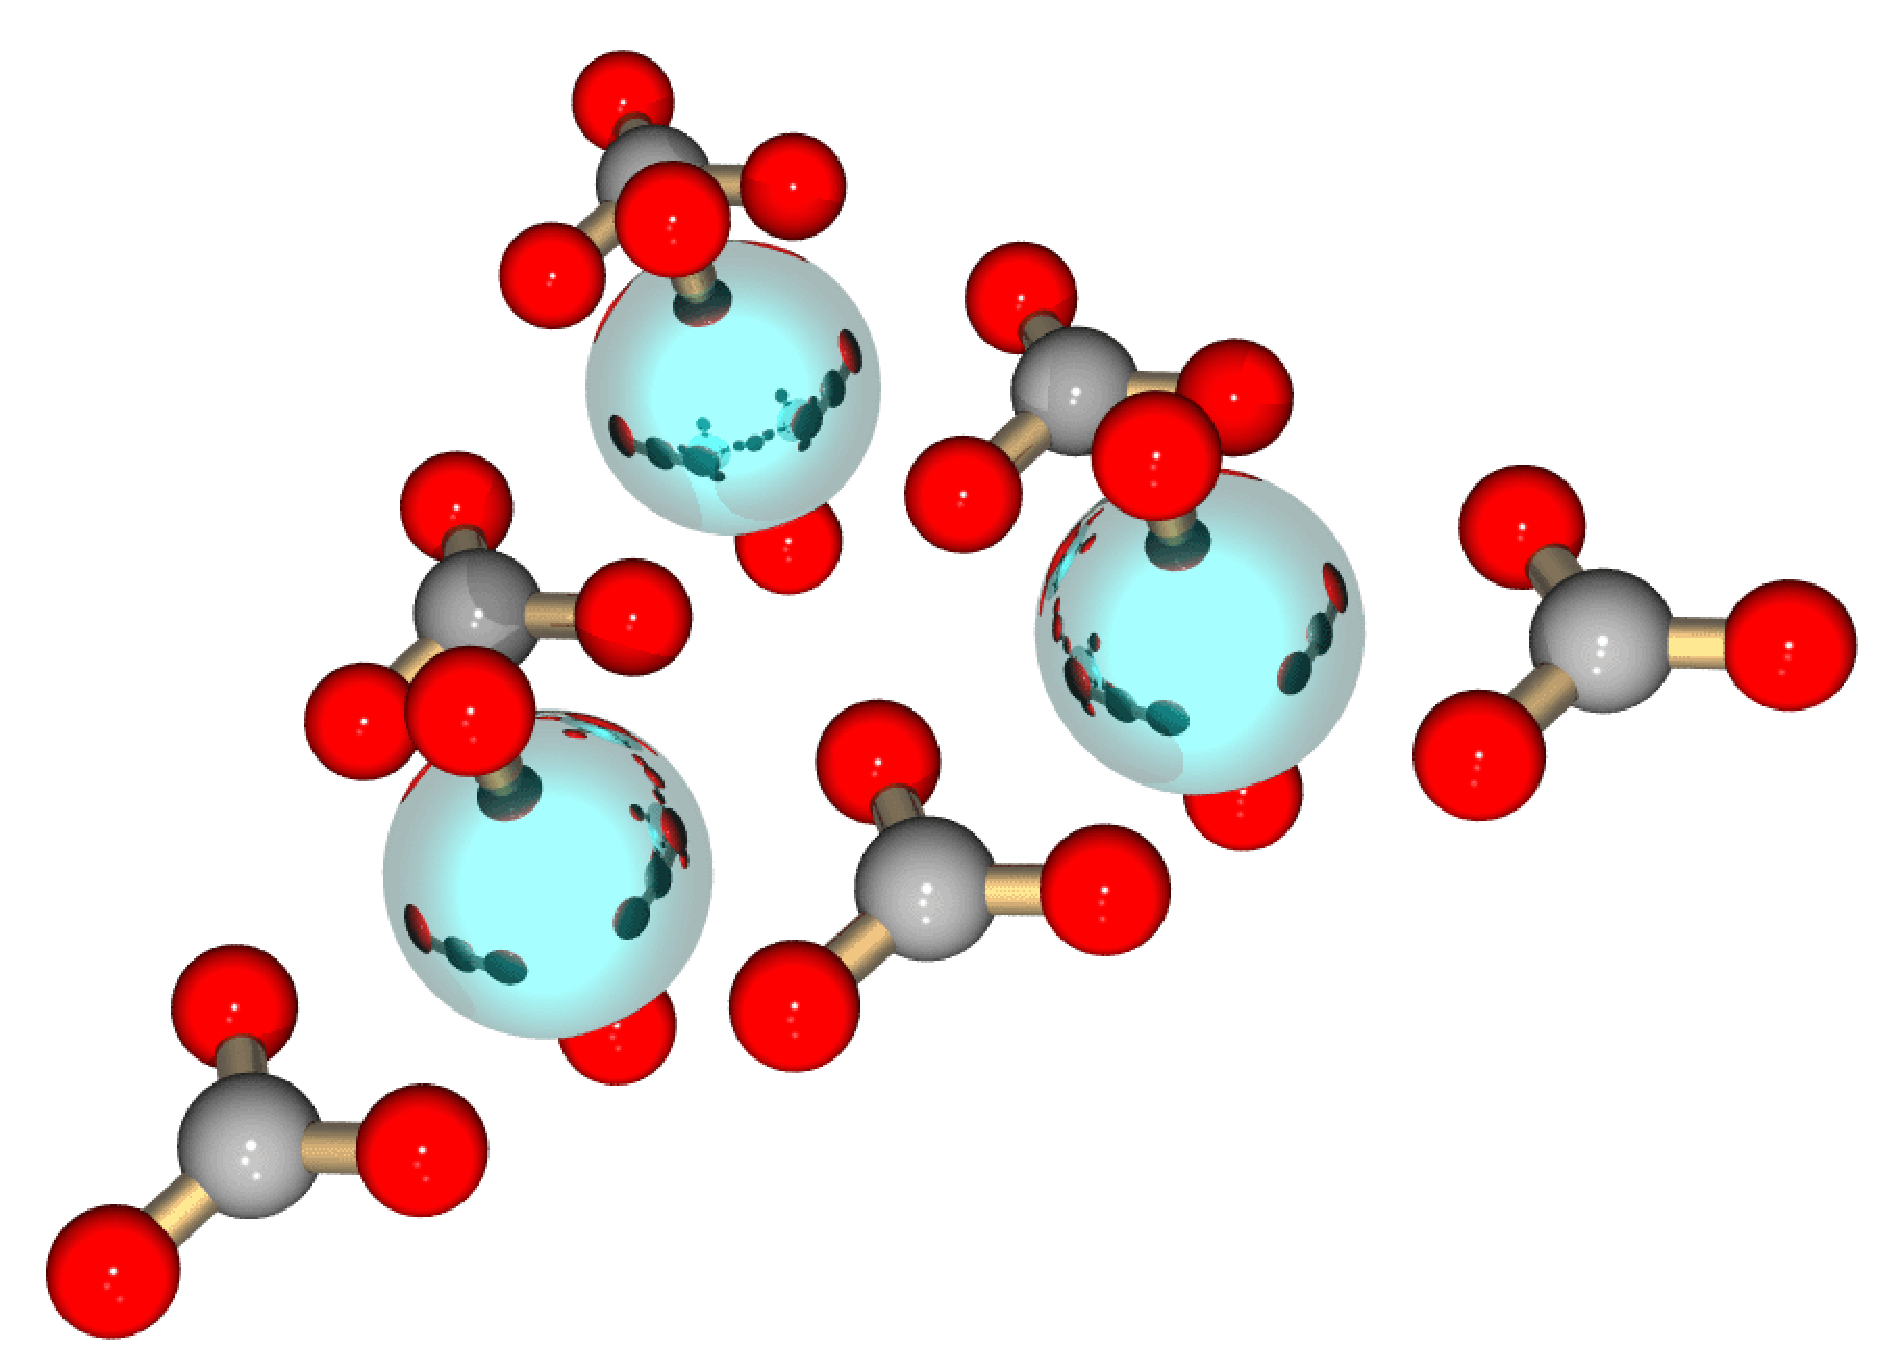
\includegraphics[height=1.2in]{../images/molecule-uo23co36}
\small
\centerline{Electronic structure optimization}
\else
\fi
\end{minipage} 
\hfil
\begin{minipage}[b]{.45\linewidth}
\ifpdf
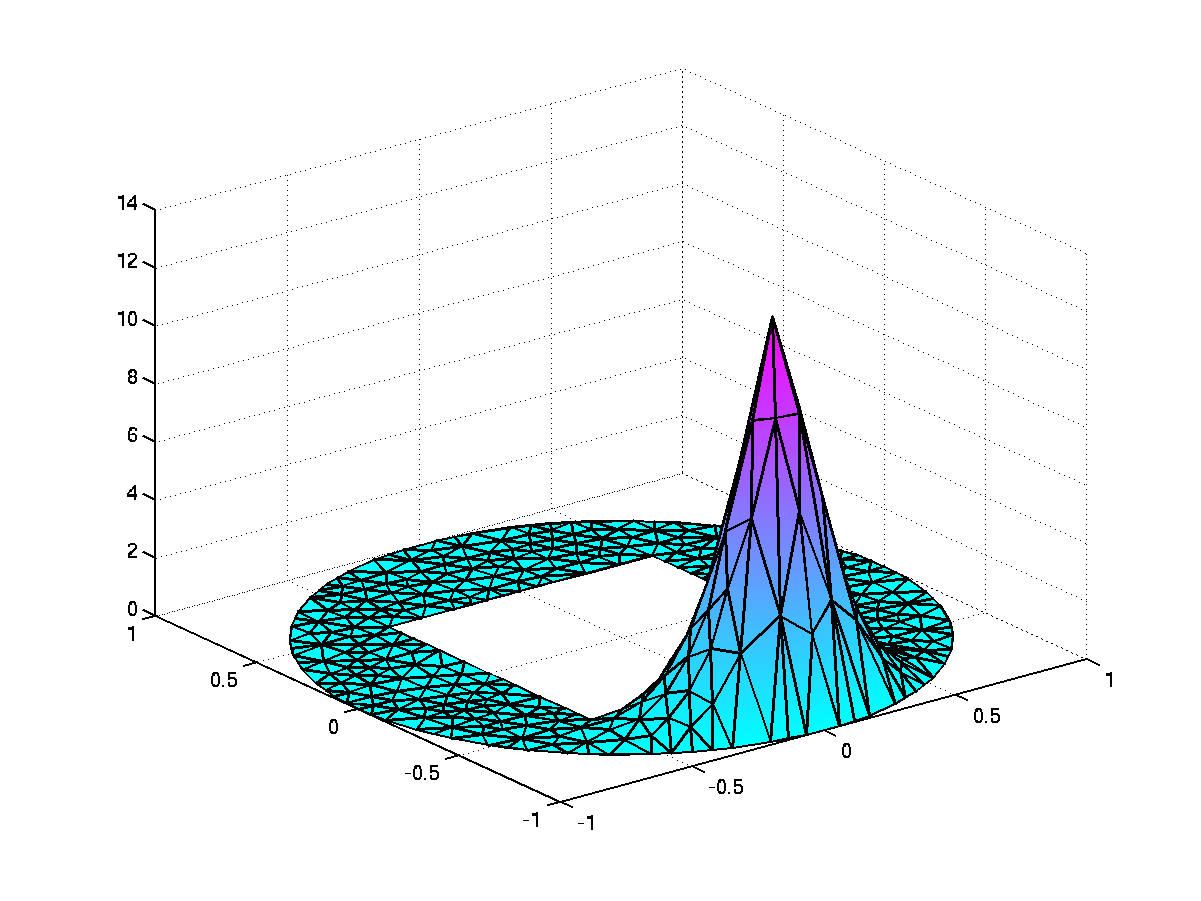
\includegraphics[height=1.4in]{../images/henon_circ_sol}
\small
\centerline{Mesh-based optimization}
\else
\fi
\end{minipage}

\bigskip
\small
\textbf{Note.} Image of $ (UO_2)_3 (CO_3)_6 $ courtesy of Wibe deJong (PNNL)

\vfill

\end{slide}

\begin{slide}

\heading{Outline}

\begin{list}{\reddiamond}{}
\item
TAO - Recent Developments
\item
Optimization applications
\item
TAO algorithms
\item
Performance for Grid Sequencing -- Stalking optimality
\item
Using TAO
\end{list}

\vfill

\end{slide}

\begin{slide}

\heading{TAO: Toolkit for Advanced Optimization}

\begin{quote}
The process of nature by which all things change
and which is to be followed for a life of harmony.  
\end{quote}


\bigskip

\begin{list}{\reddiamond}{}
\item
Object-oriented techniques
\item
Component-based interaction
\item
Leverage of existing parallel computing infrastructure
\item
Reuse of external toolkits (linear solvers, preconditioners, \ldots)
\end{list}

\vfill

\end{slide}

\begin{slide}

\heading{TAO: Recent Developments}

\begin{list}{\reddiamond}{}
\item
Version 1.5 (January 2003)
\item
Source code, documentation, tutorials, 
example problems, \ldots
\item
Development of BLMVM
\item
TAO components: MPQC (Sandia) and NWChem (PNNL)
% \item
% GA and Tao Components
\item
Grid sequencing via Distributed Arrays (PETSc)
\item
Gradients of grid functions via ADIC
\end{list}

\bigskip

\textbf{Powered by PETSc and ADIC!}

\vfill

\end{slide}

\begin{slide}

\heading{The Ginzburg-Landau Model for Superconductivity}

Minimize the Gibbs free energy
 
% for a homogeneous superconductor with a vector
% potential perpendicular to the superconductor.
{\small
\[
\int _ {\cD} \bigl \{ - | v (x) |^2 + \half | v (x) |^4  + 
\left \| \left [ \nabla - i A(x) \right ] v (x) \right \| ^2  +  \\
\kappa^2 \left \| ( \grad \times A ) (x) \right \| ^2 \bigr \} dx
\]
}
%
\begin{minipage}[b]{.45\linewidth}
Order parameter $ v : \R^2 \to \C$ 
Vector potential $A : \R^2 \to \R^2 $    
 \vspace{4em}
\end{minipage} 
\hfil 
\begin{minipage}[b]{.45\linewidth}
\centerline{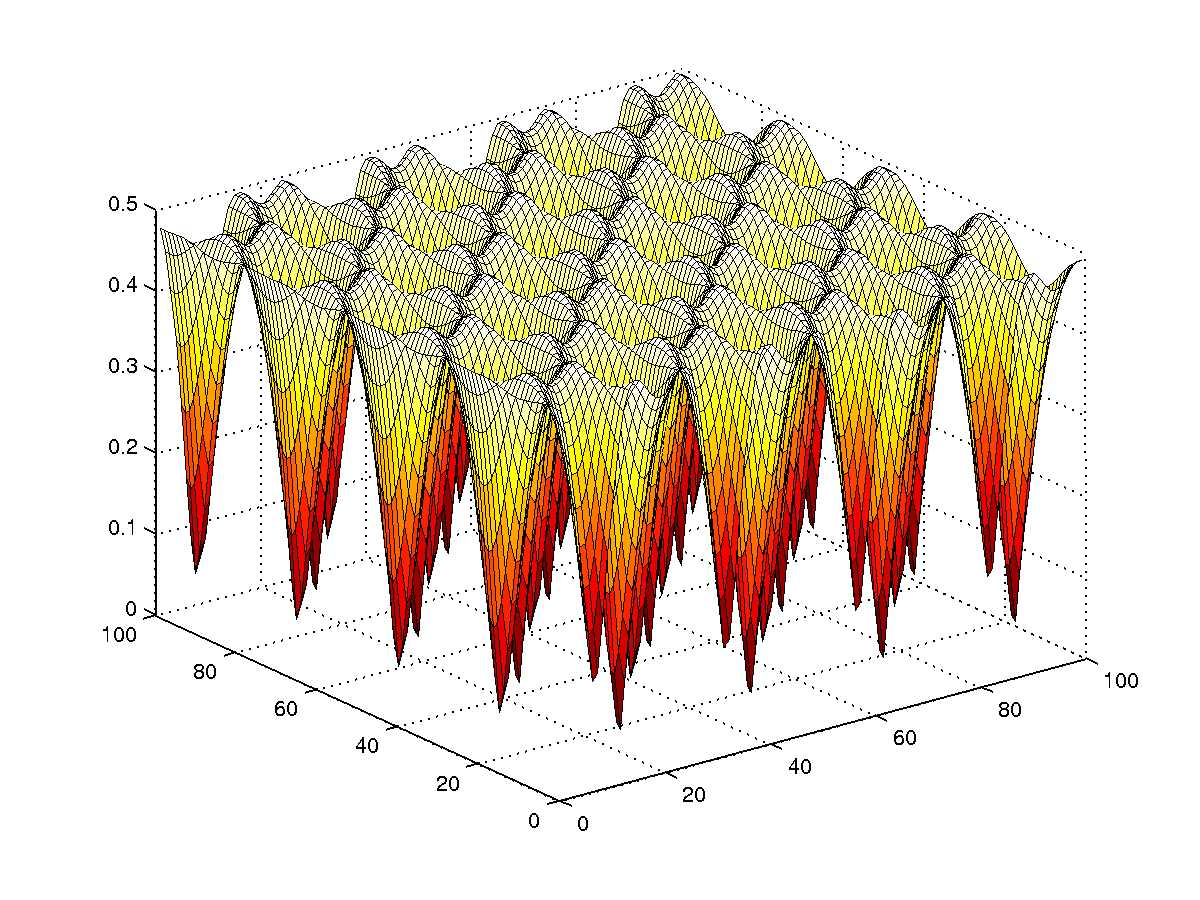
\includegraphics[width=1.7in]{../images/gl2}}
\end{minipage}

Non-convex function. Hessian is singular.
Unique minimizer. % , but there is a saddle point.

\vfill

\end{slide}

\begin{slide}

\heading{Minimal Surface with Obstacles}

\[
\min 
\left \{
\int_{ \cD } \sqrt { 1 + \| \grad v (x) \| ^ 2 } \, d x : v \ge v_L
\right \}
\]

\medskip

\begin{center}
\ifpdf
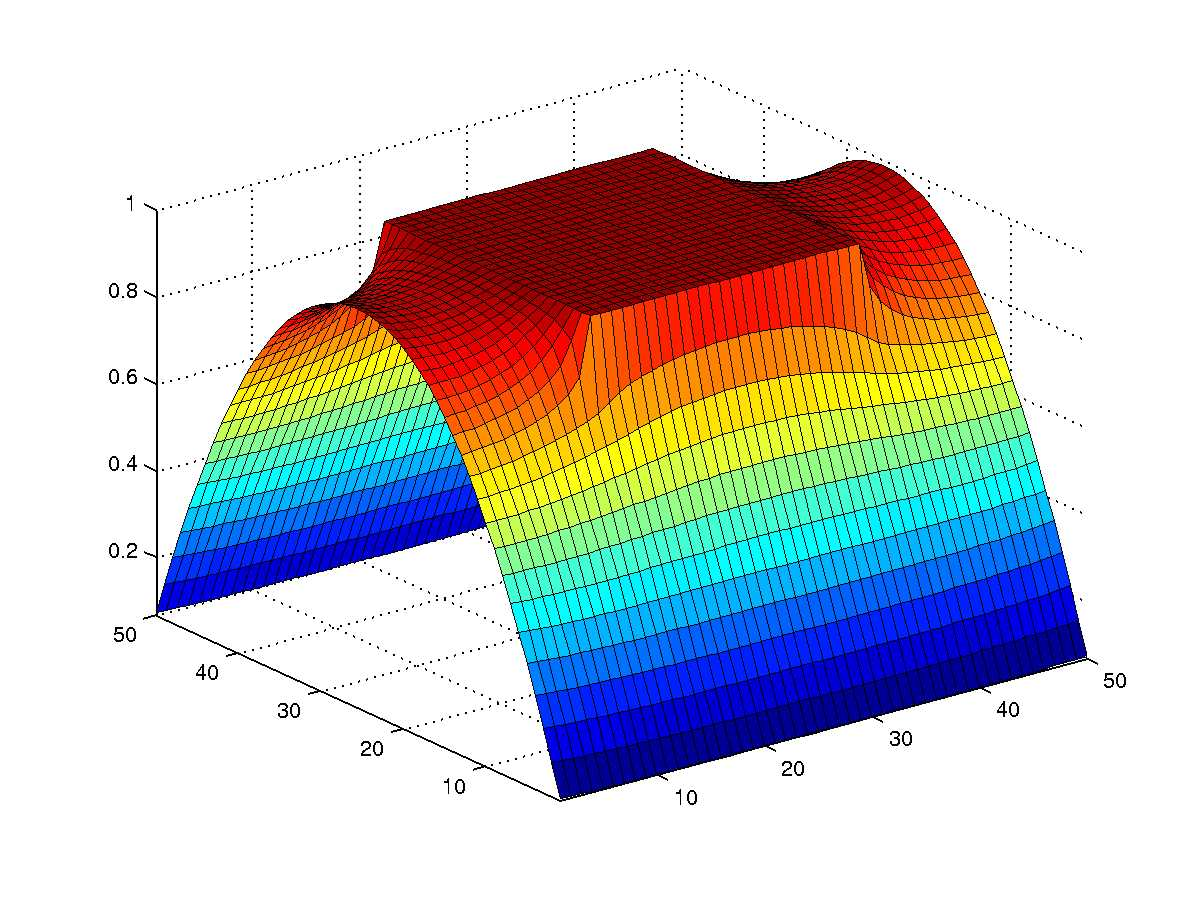
\includegraphics[height=1.2in]{../images/mso_s}
\qquad
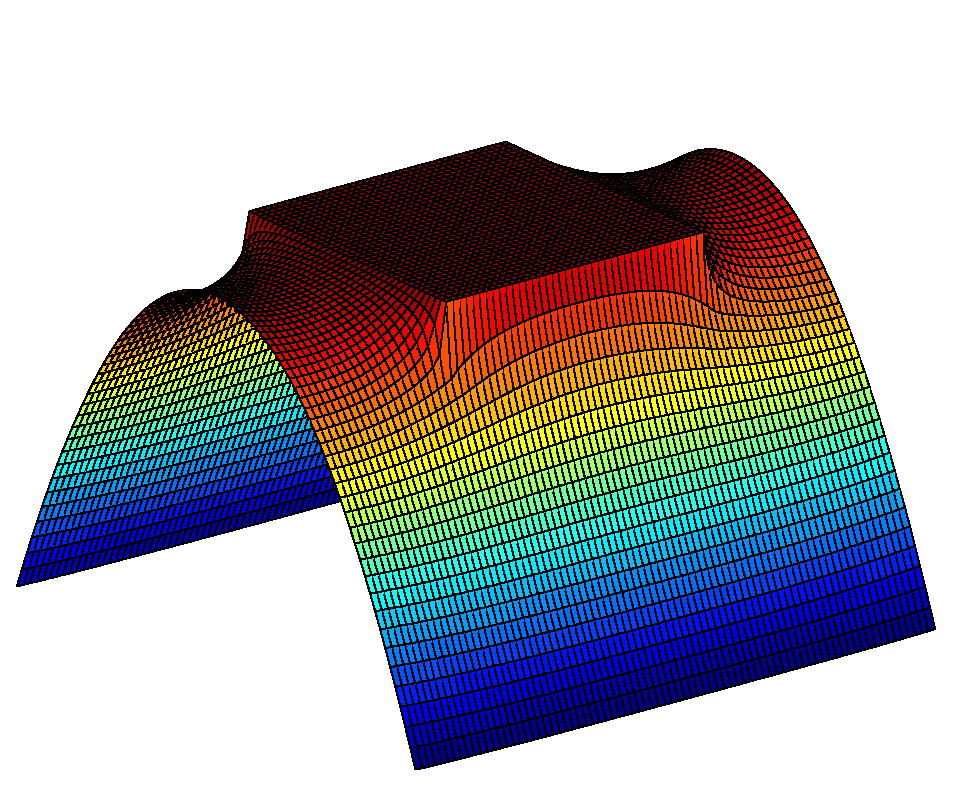
\includegraphics[height=1.2in]{../images/mso_e}
\else
\fi
\end{center}

\bigskip

Number of active constraints depends on the height of the
obstacle. The solution $ v \notin C^1 $.
Almost all multipliers are zero. 

\vfill

\end{slide}

\begin{slide}

\heading{Isomerization of $ \alpha $-pinene}

Determine the reaction coefficients
% in the thermal isometrization of $\alpha$-pinene from measurements 
by minimizing
\[
\sum _ {j=1}^8 \| y ( \tau_j ; \theta ) - z_j \| ^ 2 ,
\]
where $z_j$ are the measurements and

\begin{minipage}[b]{.45\linewidth}
\begin{eqnarray*}
y_1'  & = & -(\theta_1 + \theta_2) y_1 \\
y_2'  & = & \theta_1 y_1 \\
y_3'  & = & \theta_2 y_1 - (\theta_3 + \theta_4 )y_3 + \theta_5 y_5 \\
y_4'  & = & \theta_3 y_3 \\
y_5'  & = & \theta_4 y_3 - \theta_5 y_5  \\
\end{eqnarray*}
\end{minipage} 
\hfil 
\begin{minipage}[b]{.45\linewidth}
\centerline{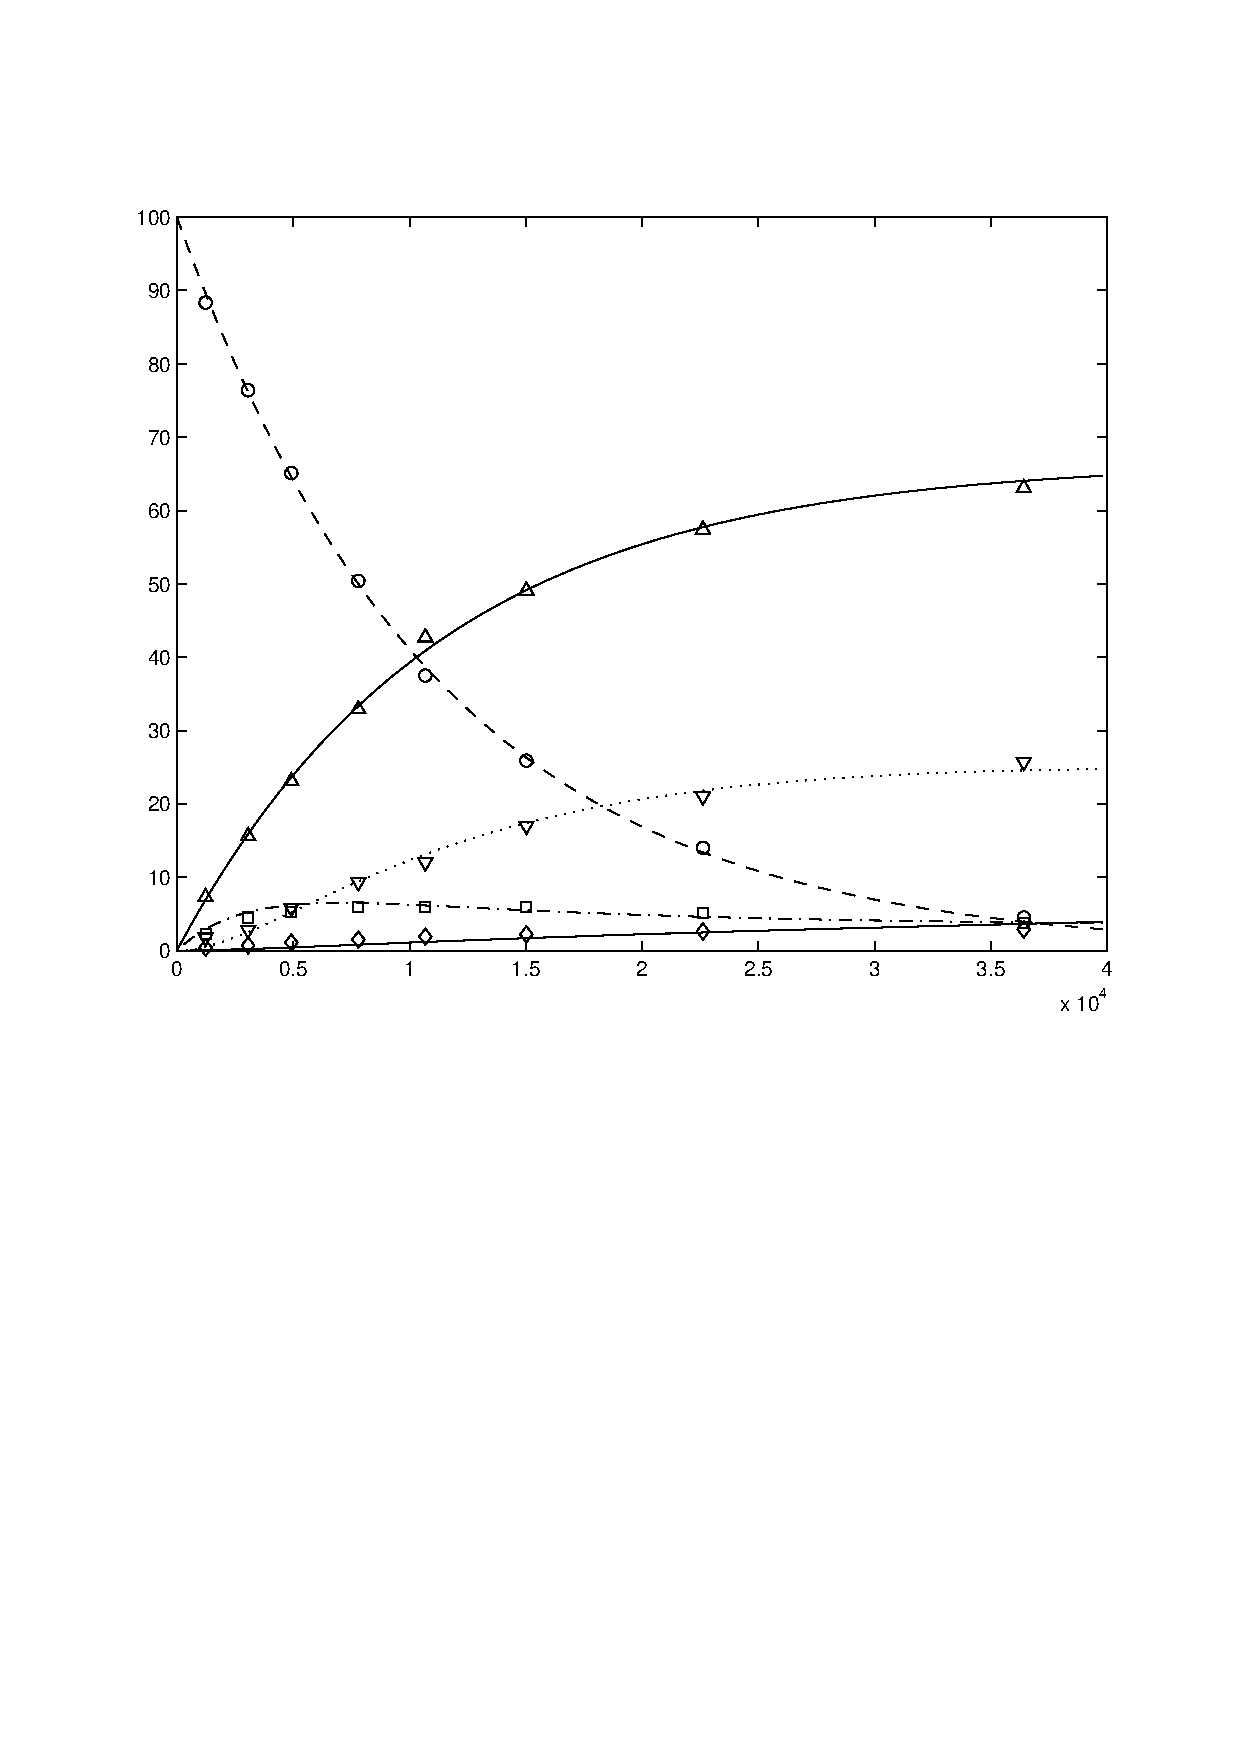
\includegraphics[width=1.4in]{../images/pinene}}
\end{minipage}

% Only equality constraints. Typical parameter estimation problem. 

\vfill

\end{slide}

\begin{slide}

\heading{Hang Glider}

Maximize the final position of a glider whose flight has
a thermal updraft at 250 meters.
The equations of motion are
\[
x''  =  \frac{1}{m}(-L\sin (\eta )-D\cos (\eta )) , \qquad
y''  =  \frac{1}{m}(L\cos (\eta )-D\sin (\eta )) - g ,
\]
where $ ( x, y ) $ is the position, $m$ is the mass, and
% of the glider, and $g$ is the gravitational constant.
% In this problem

\begin{minipage}[b]{.30\linewidth}
\begin{small}
\begin{eqnarray*}
\eta &=& \eta (x,x',y') \\
L    &=& L(x,x',y',c_L) \\
D    &=& D(x,x',y,'c_L) 
\end{eqnarray*}
\centerline{$ 0 \le c_L(t) \le c_M $}
\end{small}
\end{minipage} 
\hfil 
\begin{minipage}[b]{.30\linewidth}
\centerline{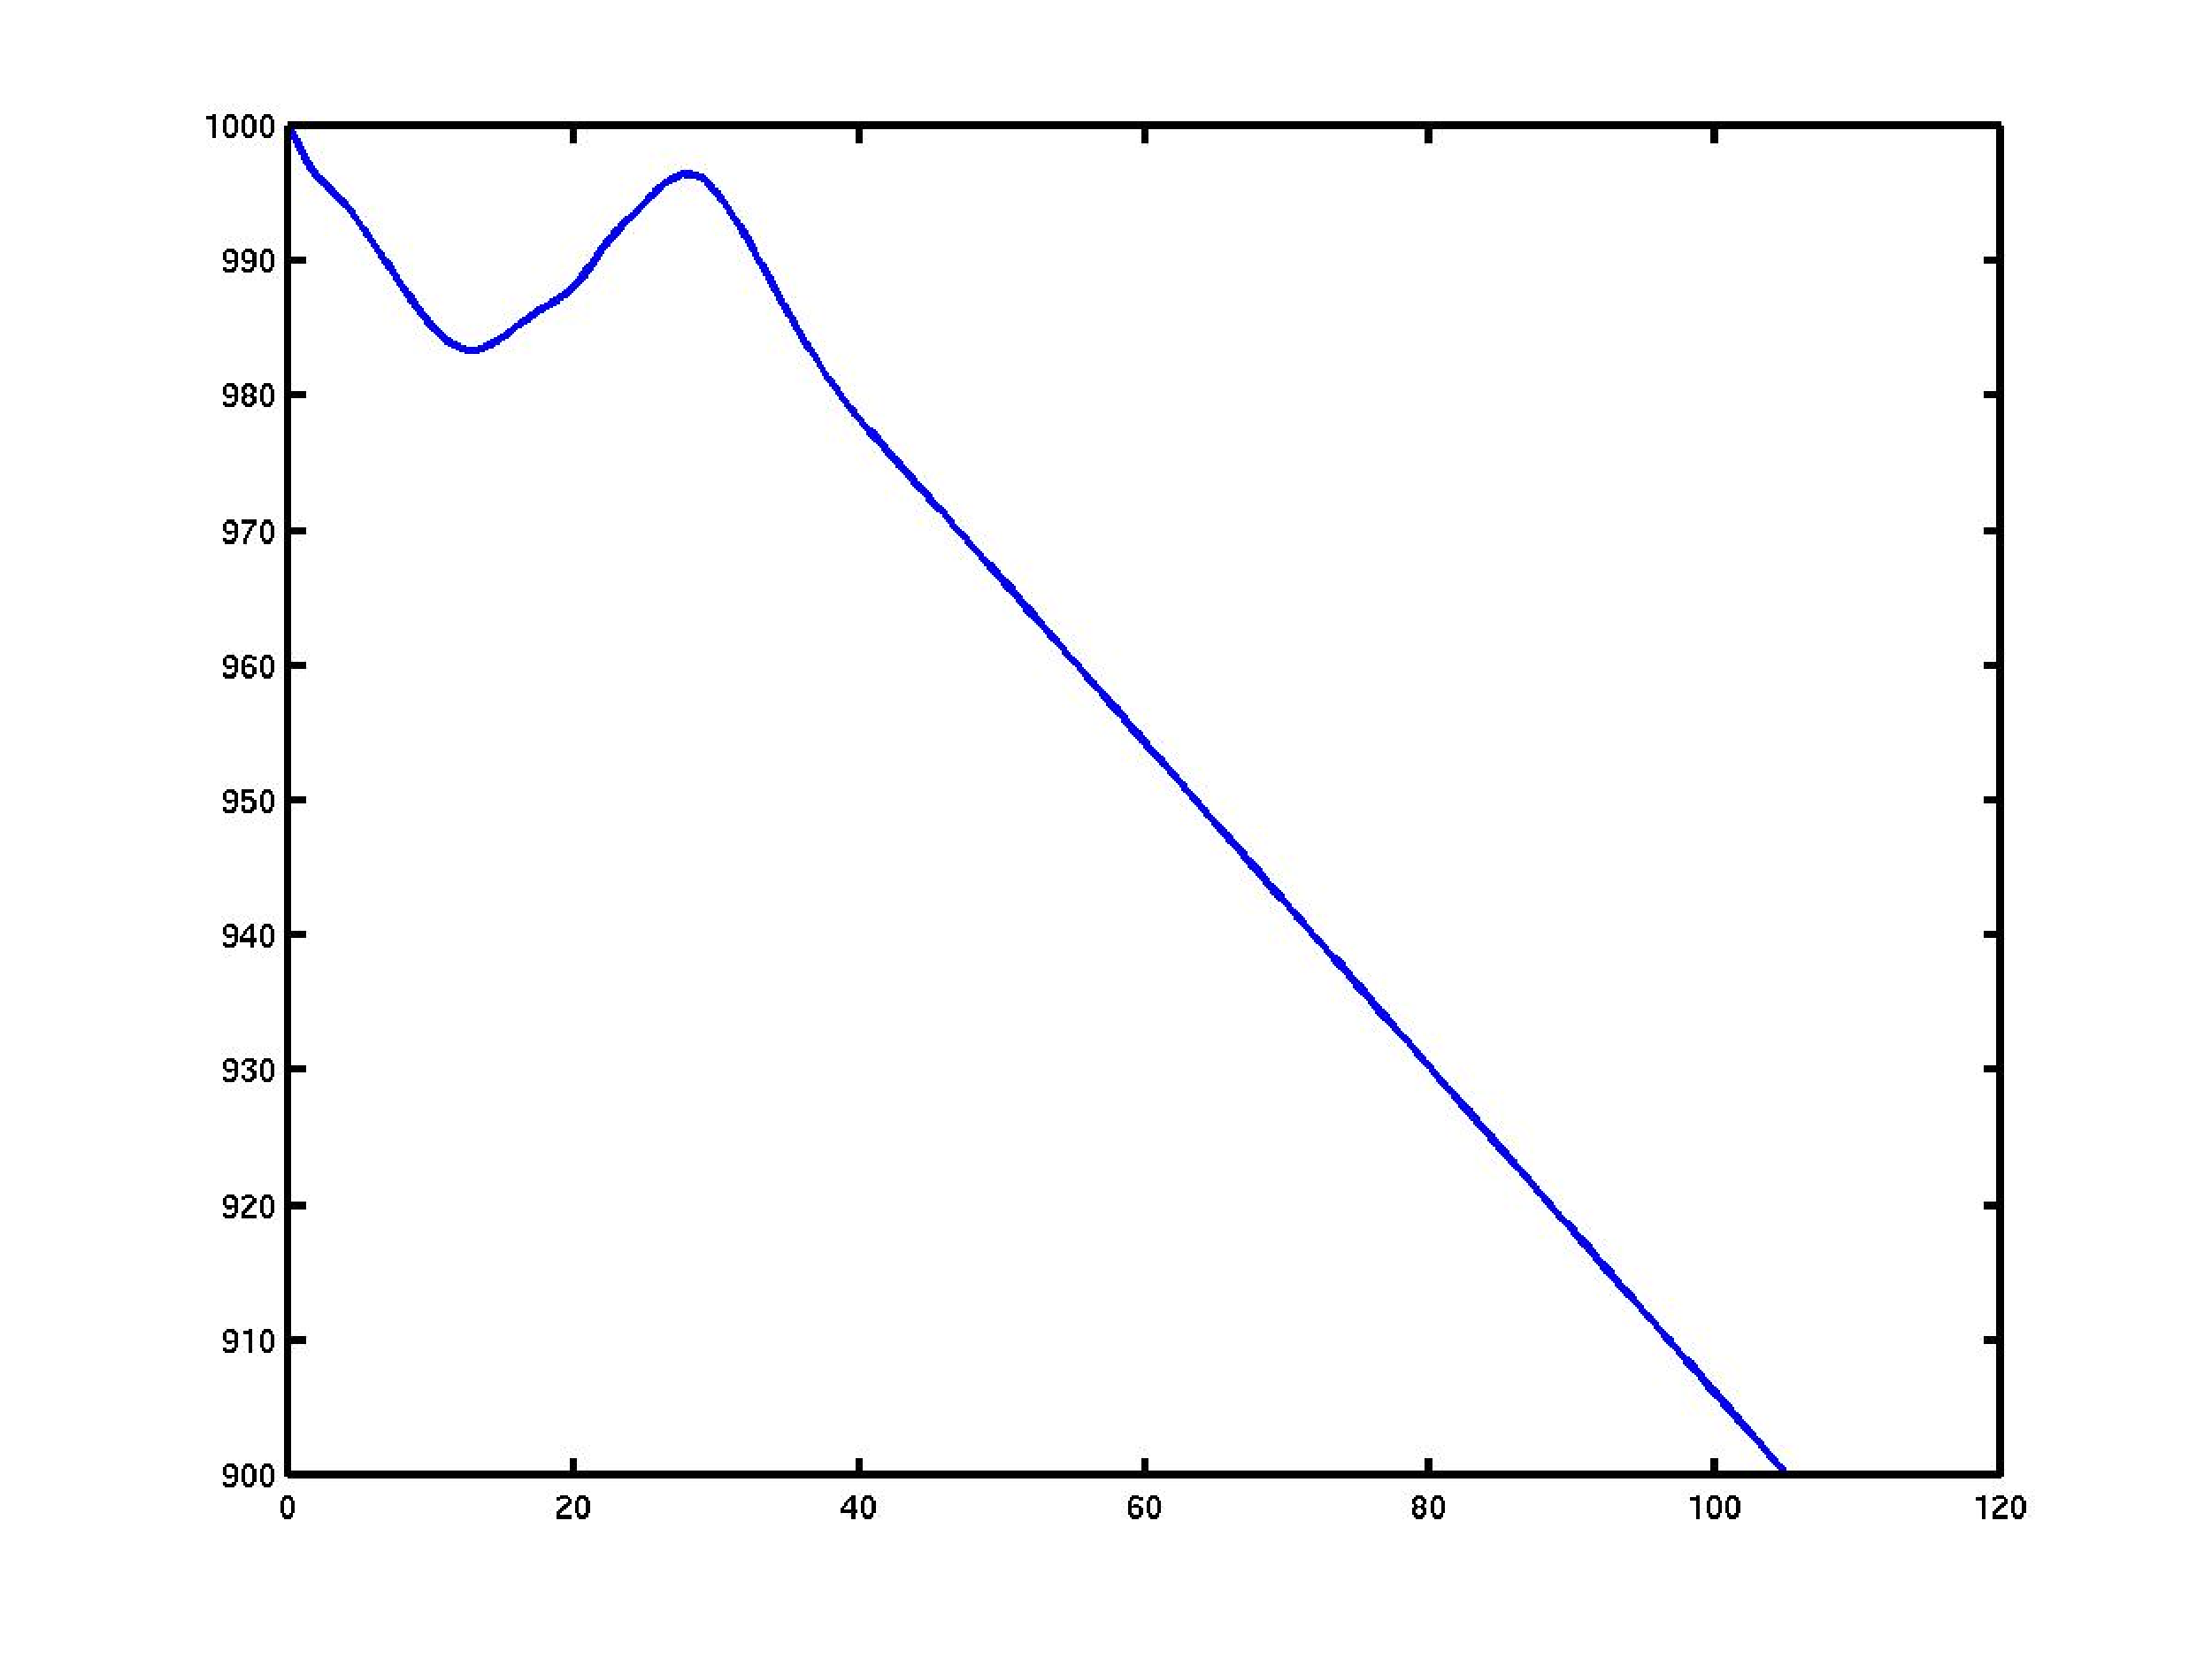
\includegraphics[width=1.4in]{../images/glider_x2}}
\end{minipage}
\hfil
\begin{minipage}[b]{.30\linewidth}
\centerline{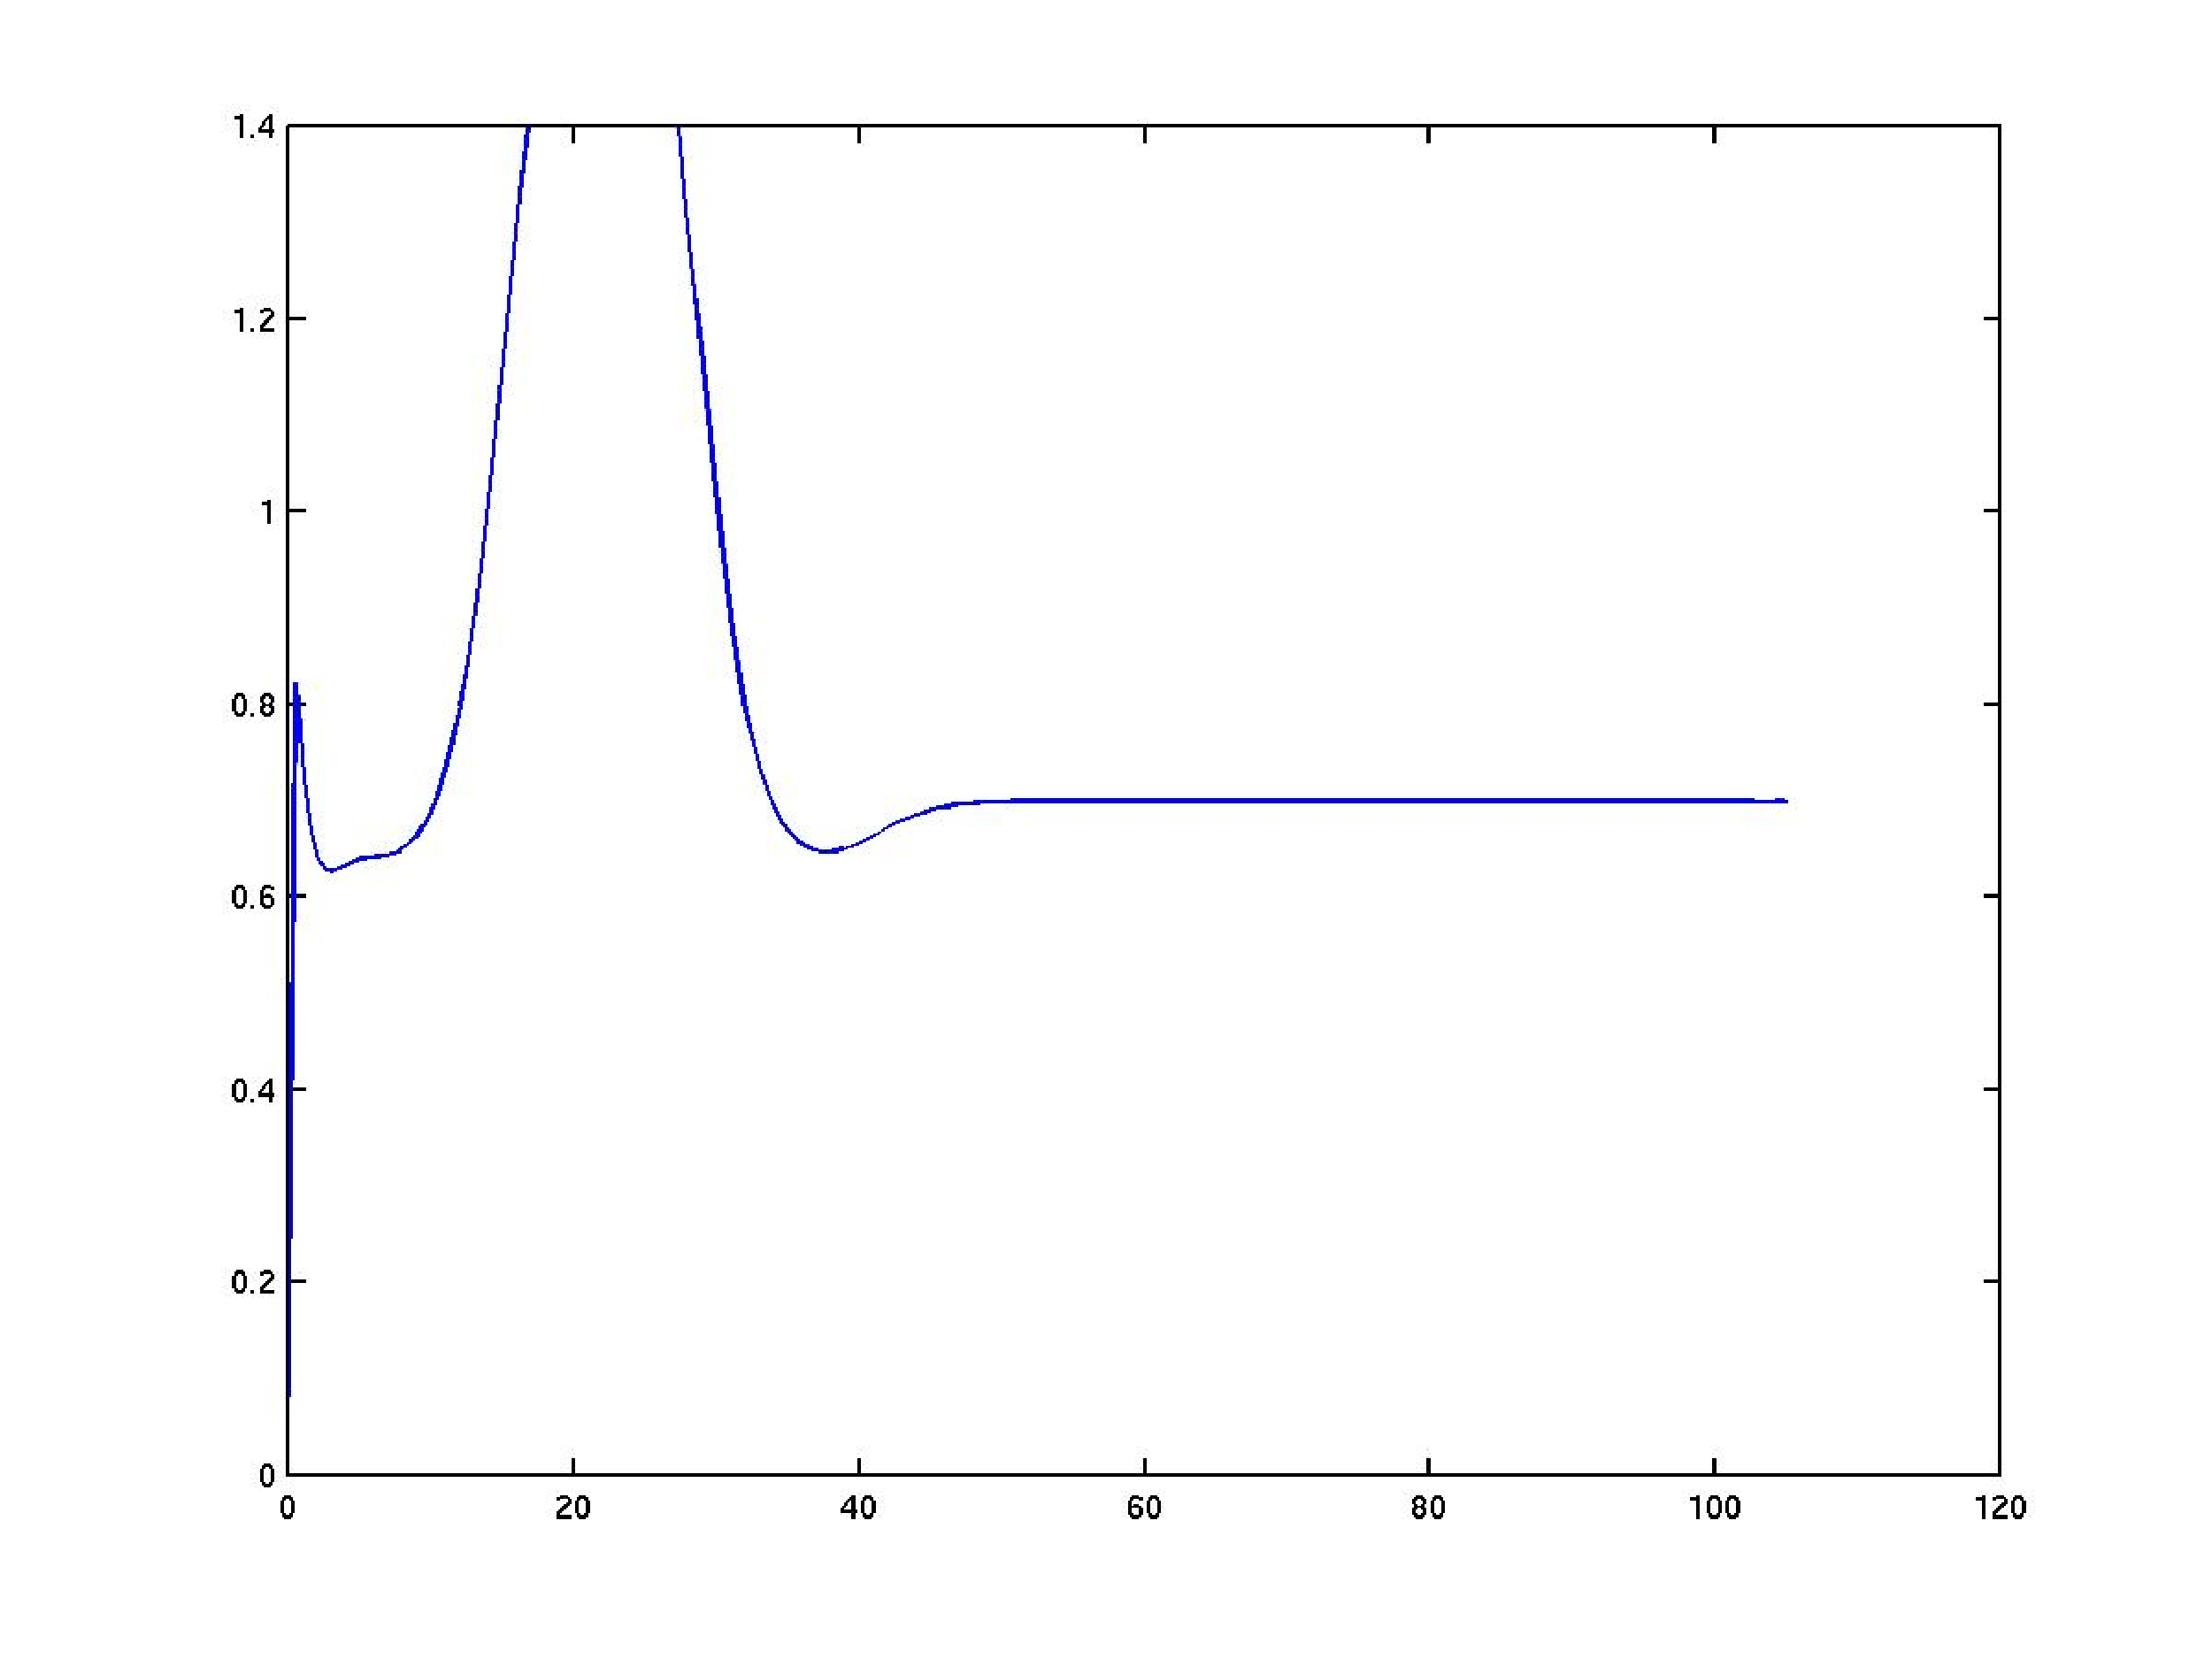
\includegraphics[width=1.4in]{../images/glider_cl}}
\end{minipage}

The control  (drag) $ c_L $ is not differentiable at the
switching points.

\vfill

\end{slide}

\begin{slide}

\heading{Transition States}

Given a continuously differentiable function  $ f : \R^n \mapsto \R $ 
and two points $ x_a $ and $ x_b $, 
determine a critical point $ x^* $
on a minimal energy path between $ x_a $ and $ x_b $.

\medskip

\redball \quad A fundamental problem in biology, chemistry, and mathematics

\bigskip

\begin{minipage}[b]{.60\linewidth}
\begin{small}
A critical value of $f$ is
\[
\gamma =  \inf_{p \in \Gamma} 
\left \{ \max \left \{ f[p(t)] : t \in [0,1] \right \} \right \} 
\]
when $ \Gamma $ is defined by
\[
\Gamma = \left \{ p \in C [0,1] : p(0) = x_a , \ p(1) = x_b \right \} .
\]
\end{small}
\end{minipage} 
\hfil
\begin{minipage}[b]{.35\linewidth}
\ifpdf
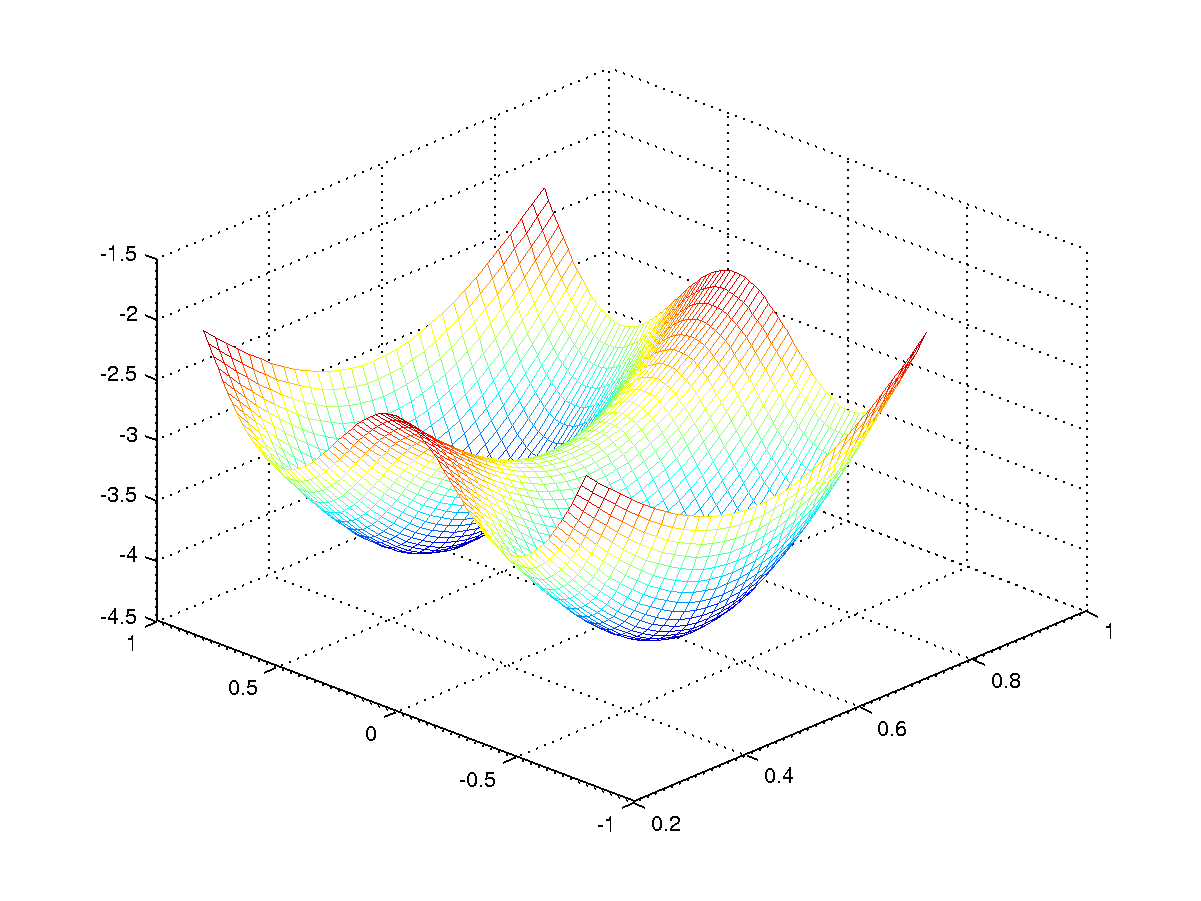
\includegraphics[height=1.3in]{../images/gaussian}
\else
\fi
\end{minipage}

\vfill

\end{slide}

\begin{slide}

\heading{The Elastic String Algorithm}

Compute breakpoints $ x_k \in \R^n $ for a piecewise linear path such that
\[
\min \left \{ \max \left \{ f (x_1) , \ldots , f(x_m) \right \}
: \| x_{k+1} - x_k \| \le h_k , 
\ 0 \le k \le m \right \} .
\]
% \[
% \| x_{k+1} - x_k \| \le h_k , \qquad \sum _{k=0}^{m} h_k = L ,
% \]
% and $ \sum _{k=0}^{m} h_k = L $, and
% $ L $ is a bound on the length of the path.

\bigskip

\ifpdf
\centerline{
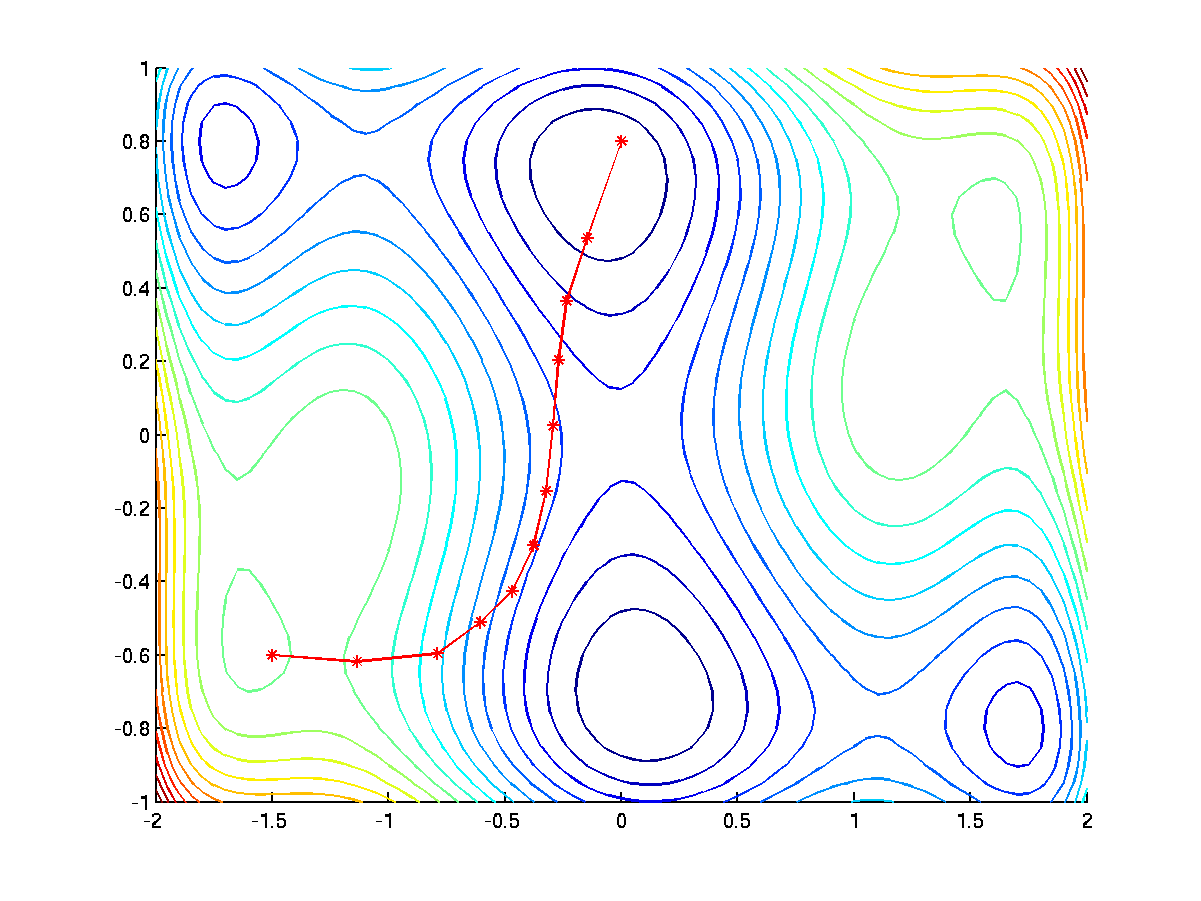
\includegraphics[height=1.7in]{../images/camel10} \hfil
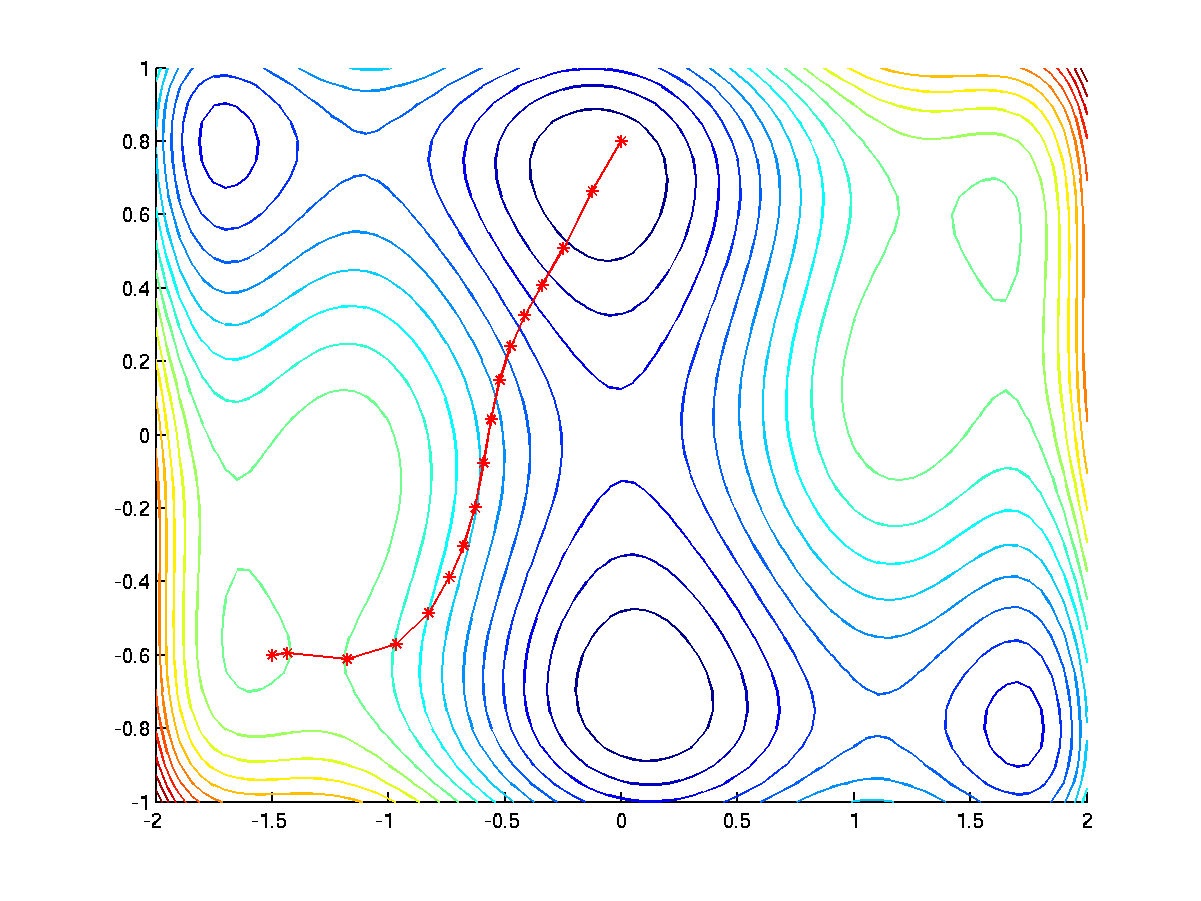
\includegraphics[height=1.7in]{../images/camel15}
}
\else
\fi

\vfill

\end{slide}

\begin{slide}

\heading{TAO Algorithms for Bound-Constrained Optimization}

\[
\min \left \{  f(x) : x_l \le x \le x_u \right \}
\]

\medskip

\begin{list}{\reddiamond}{}
\item
Conjugate gradient algorithms
\item
Limited-memory variable-metric algorithms
\item
Newton algorithms
\end{list}

You must supply the function $ f : \R^n \mapsto \R $ and the
gradient 
\[
\grad f (x) = \left ( \partial _i f(x) \right )
\]

For Newton methods you also need to supply the Hessian matrix.
\[
\grad^2 f (x) = \left ( \partial_{i,j} f(x) \right )
\]

\vfill

\end{slide}

\begin{slide}

\heading{Conjugate Gradient Algorithms}

\[
x_{k+1} = x_k + \alpha_k p_k 
\]
\[
p_{k+1} = - \grad f (x_k) + \beta_k p_k 
\]
where $ \alpha_k $ is determined by a line search.

\medskip

Three choices of $ \beta_k $ are possible ($ g_k = \grad f (x_k ) $):
 
\[
\beta_k^{FR} = \left (
\frac{\| g_{k+1} \|}{\| g_k \|}
\right ) ^ 2 , \qquad \mbox{Fletcher-Reeves}
\]
\[
\beta_k^{PR} = 
\frac{ \langle g_{k+1} , g_{k+1} - g_k \rangle }
{\| g_k \|^2},  \qquad \mbox{Polak-Rivi\`ere}
\]
\[
\beta_k^{PR+} = \max \left \{ \beta_k^{PR} , 0 \right \} , \qquad
\mbox{PR-plus}
\]

\vfill

\end{slide}

\begin{slide}

\heading{Limited-Memory Variable-Metric Algorithms}

\[
x_{k+1} = x_k - \alpha_k H_k \grad f (x_k )
\]
where $ \alpha_k $ is determined by a line search.

\medskip 

The matrix $ H_k $ is defined in terms
of information gathered during the
previous $m$ iterations.

\medskip

\begin{list}{\reddiamond}{}
\item
$ H_k $ is positive definite.
\item
Storage of $ H_k $ requires $ 2 m n $ locations.
\item
Computation of $ H_k \grad f (x_k) $ costs
$ (8m+1) n $ flops.
\end{list}

\vfill

\end{slide}

\begin{slide}

\heading{Trust Region Newton Algorithm}

At each iteration the step $s_k$  (approximately) minimizes 
\[
\min 
\left \{ 
q_k ( x_k + s ) : s_i = 0, \ i \in \cA_k , \
x_l \le x_k + s \le x_u , \ \| s \| \le \Delta_k 
\right \}
\]
where $ q_k $ is the quadratic approximation,
\[
q_k (w) = \langle \grad f (x_k ) , w \rangle + 
\half \langle w , \grad ^2 f(x_k) w \rangle ,
\]
to the function, and $ \Delta_k $ is the trust region bound.
\medskip

\begin{list}{\reddiamond}
{
\setlength{\itemsep}{0pt}
\setlength{\parsep}{0pt}
}
\item
Predict an active set $ \cA_k $.
\item
Compute a step $ s_k $ 
\item
$ x_{k+1} = x_k + s_k $ if $ f (x_k + s_k ) < f (x_k) $, 
otherwise $ x_{k+1} = x_k $.
\item
Update $ \Delta_k $.
\end{list}

\vfill

\end{slide}

\begin{slide}

\heading{Mesh Sequencing Issues}

\begin{list}{\reddiamond}{}
\item[\redball]
How much does mesh-sequencing save?
\item[\redball]
Does mesh-sequencing resolve the convergence issue?
\item
What is the order of convergence of $ f ( x_h^*) $?
\item
What is the order of convergence of $ x_h^* $?
\item
How does the number of active constraints at $ x_h $ change?
\item
What tolerance do we use to obtain $ x_h $?
\item
What is the impact on iterative methods on these results?
\end{list}

\vfill

\end{slide}

\begin{slide}

\heading{TAO Benchmark: Pressure in a Journal Bearing}

\[
\min 
\left \{
\int_{ \cD } \left \{ \half  w_q (x) \| \grad v (x) \| ^ 2  -
  w_l (x) v (x) \right \} \, d x : v \ge 0
\right \}
\]
%
\begin{minipage}[b]{.45\linewidth}
\[
\begin{array}{c}
 w_q ( \xi_1 , \xi_2 ) = ( 1 + \epsilon \cos \xi_1 ) ^ 3  \\
 w_l ( \xi_1 , \xi_2 ) = \epsilon \sin \xi_1 \\
 \cD = ( 0 , 2 \pi ) \times ( 0 , 2b ) 
\end{array}
\]
\vspace{0.5em}
\end{minipage} \hfil
\begin{minipage}[b]{.45\linewidth}
\ifpdf
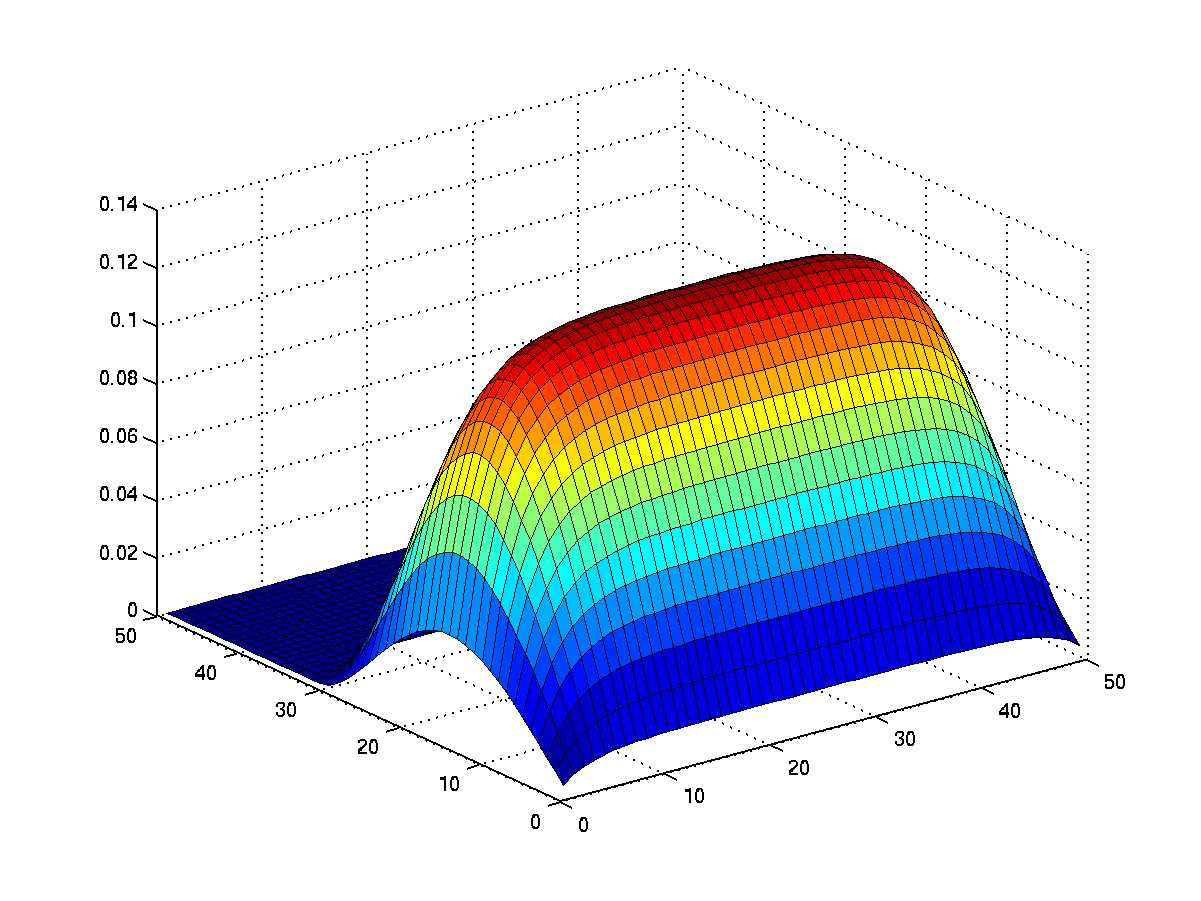
\includegraphics[height=1.2in]{../images/pjb5050}
\else
\fi
\end{minipage}

\medskip

Number of active constraints depends on the choice of 
$ \epsilon $ in $ (0,1) $.  \\
Nearly degenerate problem. Solution $ v \notin C^2 $.

\vfill

\end{slide}

\begin{slide}

\heading{TAO Benchmark: Minimal Surface with Obstacles}

\[
\min 
\left \{
\int_{ \cD } \sqrt { 1 + \| \grad v (x) \| ^ 2 } \, d x : v \ge v_L
\right \}
\]

\medskip

\begin{center}
\ifpdf
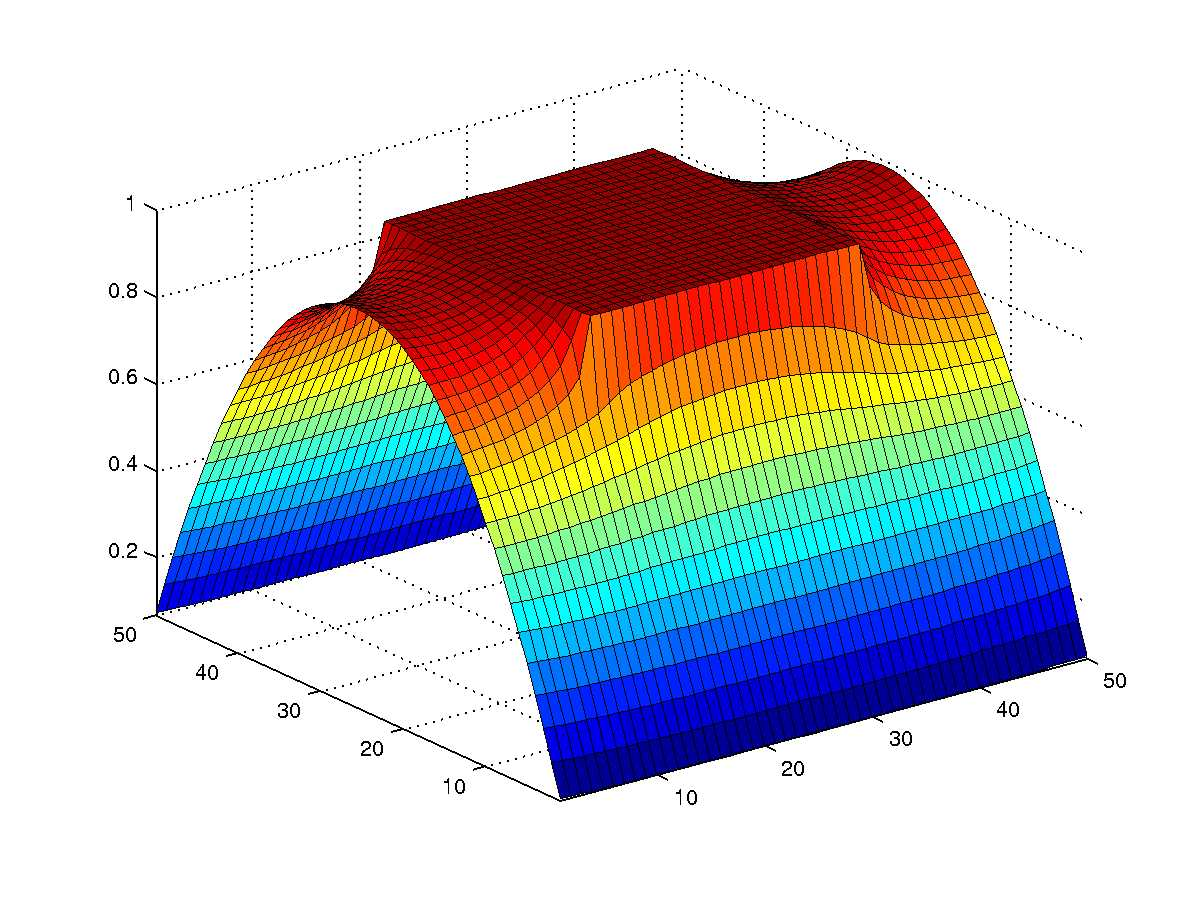
\includegraphics[height=1.2in]{../images/mso_s}
\qquad
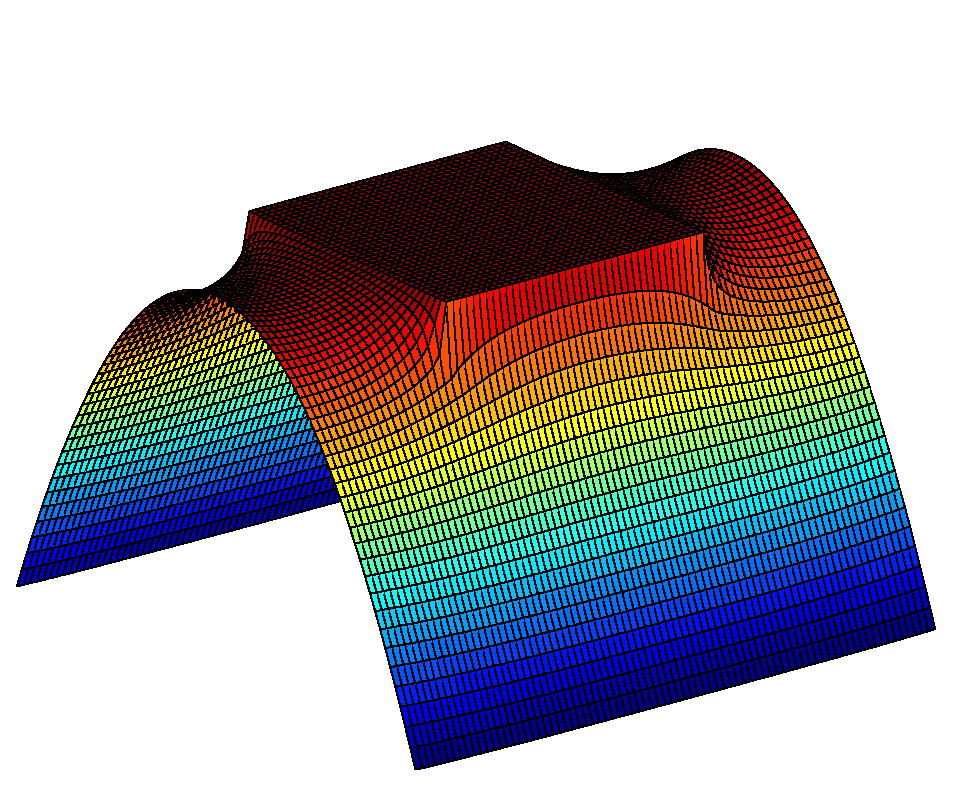
\includegraphics[height=1.2in]{../images/mso_e}
\else
\fi
\end{center}

\bigskip

Number of active constraints depends on the height of the
obstacle. The solution $ v \notin C^1 $.
Almost all multipliers are zero. 

\vfill

\end{slide}

\begin{slide}

\heading{Mesh-Sequencing Performance: Journal Bearing Problem}

\begin{center}
\begin{tabular}{ccccccc}
      & \multicolumn{6}{c}{Number of processors} \\ \cline{2-7}
      &  \multicolumn{2}{c}{16} & \multicolumn{2}{c}{32} &
         \multicolumn{2}{c}{64} \\  \cline{2-7}
 Mesh & $ \boxplus $ & $ \square $ & $ \boxplus $ & $ \square $ & $ \boxplus $ & $ \square $ \\
\hline
 769 $\times$  769  &  17  &   283  &   10   &   142   &    7  &   86 \\
1537 $\times$  1537 &  73  &  3751  &   40   &  1861   &   22  &  938 \\
\hline
\end{tabular}
\end{center}

\bigskip\bigskip

\textbf{Improvements} \qquad \qquad 
\begin{tabular}{cccc}
%      & \multicolumn{3}{c}{Number of processors} \\ \cline{2-4}
 Mesh &  16  &  32  &  64  \\
\hline
 769 $\times$  769  &  16  &  14  & 12 \\
1537 $\times$  1537 &  51  &  46  & 42  \\
\hline
\end{tabular}

\vfill

\end{slide}

\begin{slide}

\heading{Mesh-Sequencing Performance: Obstacle Problem}

\begin{center}
\begin{tabular}{ccccccc}
      & \multicolumn{6}{c}{Number of processors} \\ \cline{2-7}
      &  \multicolumn{2}{c}{16} & \multicolumn{2}{c}{32} &
         \multicolumn{2}{c}{64} \\  \cline{2-7}
 Mesh & $ \boxplus $ & $ \square $ & $ \boxplus $ & $ \square $ & $ \boxplus $ & $ \square $ \\
\hline
 769 $\times$  769  &  69  & $\dagger$ &  37 & $\dagger$ &  24  & $\dagger$ \\
1537 $\times$  1537 &  444 & $\dagger$ & 235 & $\dagger$ & 121  & $\dagger$ \\
\hline
\end{tabular}
\end{center}

\bigskip\bigskip

$\dagger$ \textbf{No convergence after 500 iterations!}

\vfill

\end{slide}

\begin{slide}

\heading{Using TAO}

There are three parts of a TAO application program:
\begin{list}{\blackdiamond}{}

\item \textcolor{red}{{\bf Vector} and {\bf matrix} objects from
PETSc or other numerical packages.}

\item \textcolor{blue}{{\bf Applications} contain routines that
evaluate an objective function, define constraints on the
variables, and provide derivative information.}

\item \textcolor{green}{The {\bf TAO solver} with desired
algorithmic options and tolerances.}


\end{list}

\end{slide}

\begin{slide}
\heading{Using TAO with PETSc}
\begin{alltt}
\scriptsize \setlength{\baselineskip}{8pt}
  TAO_SOLVER      tao;              /* TAO Optimization solver          */
  TAO_APPLICATION app;              /* TAO Application using PETSc      */
  AppCtx          user;             /* user-defined application context */
  \textcolor{red}{Vec             x;                /* solution vector                  */
  Mat             H;                /* Hessian Matrix                   */}

  \textcolor{red}{VecCreateSeq(PETSC_COMM_SELF,n,&x);
  MatCreateSeqAIJ(PETSC_COMM_SELF,n,n,nz,NULL,&H);}
  TaoCreate(PETSC_COMM_SELF,''tao_lmvm'',&tao);
  TaoApplicationCreate(PETSC_COMM_SELF,&app);
  TaoAppSetInitialSolutionVec(app,x);
  TaoAppSetObjectiveRoutine(app, FormFunction,(void *)&user);
  TaoAppSetGradientRoutine(app,FormGradient,(void *)&user);
  TaoAppSetHessianMat(app,H,H);
  TaoAppSetHessianRoutine(app,FormHessian,(void *)&user);
  TaoSolveApplication(app,tao);
  VecView(x,PETSC_VIEWER_STDOUT_SELF);
\end{alltt}

\vfill

\end{slide}



\begin{slide}

\heading{Objective Function and Gradient Evaluation}

\begin{alltt}
\scriptsize \setlength{\baselineskip}{8pt}
\textcolor{blue}{
  typedef struct \{}          /* Used in the minimum surface area problem */
    \textcolor{blue}{int         mx, my;}            /* discretization in x, y directions */
    \textcolor{blue}{int         bmx, bmy, bheight;}             /* The size of the plate */
    \textcolor{blue}{double      bheight;}                     /* The height of the plate */
    \textcolor{blue}{double     *bottom, *top, *left, *right;}         /* boundary values */
  \} \textcolor{blue}{AppCtx;}

  \textcolor{blue}{int FormFunction}(\textcolor{green}{TAO_APPLICATION app}, \textcolor{red}{Vec x}, \textcolor{blue}{double *fcn}, \textcolor{blue}{void *userCtx})\{
     \textcolor{blue}{AppCtx *user = (AppCtx *)userCtx;}
     ...
  \}
  \textcolor{blue}{int FormGradient}(\textcolor{green}{TAO_APPLICATION app}, \textcolor{red}{Vec x, Vec g}, \textcolor{blue}{void *userCtx})\{
     \textcolor{blue}{AppCtx *user = (AppCtx *)userCtx;}
     ...
  \}
  \textcolor{blue}{int FormHessian}(\textcolor{green}{TAO_APPLICATION app}, \textcolor{red}{Vec x, Mat *H, Mat *H, int *flag}, \textcolor{blue}{void *userCtx})\{
     \textcolor{blue}{AppCtx *user = (AppCtx *)userCtx;}
     ...
  \}

\end{alltt}

\vfill

\end{slide}



\begin{slide}

\heading{Creating and Using a TAO Application}

\begin{alltt}
\scriptsize \setlength{\baselineskip}{8pt}
  TAO_SOLVER      tao;              /* TAO Optimization solver          */
  \textcolor{green}{TAO_APPLICATION app;              /* TAO Application using PETSc      */}
  AppCtx          user;             /* user-defined application context */
  Vec             x;                /* solution vector                  */
  Mat             H;                /* Hessian Matrix                   */

  VecCreateSeq(PETSC_COMM_SELF,n,&x);
  MatCreateSeqAIJ(PETSC_COMM_SELF,n,n,nz,NULL,&H);
  TaoCreate(PETSC_COMM_SELF,TAOLMVM,&tao);
  \textcolor{green}{TaoApplicationCreate(}\textcolor{blue}{PETSC_COMM_SELF},\textcolor{green}{&app});
  \textcolor{green}{TaoAppSetInitialSolutionVec(app},\textcolor{red}{x});
  \textcolor{green}{TaoAppSetObjectiveRoutine(app},\textcolor{blue}{FormFunction},\textcolor{blue}{(void *)&user});
  \textcolor{green}{TaoAppSetGradientRoutine(app},\textcolor{blue}{FormGradient},\textcolor{blue}{(void *)&user});
  \textcolor{green}{TaoAppSetHessianMat(app},\textcolor{red}{H},\textcolor{red}{H});
  \textcolor{green}{TaoAppSetHessianRoutine(app},\textcolor{blue}{FormHessian},\textcolor{blue}{(void *)&user});
  TaoSolveApplication(app,tao);
  VecView(x,PETSC_VIEWER_STDOUT_SELF);
\end{alltt}

\vfill

\end{slide}


\begin{slide}

\heading{Creating and Using a TAO Solver}

\begin{alltt}
\scriptsize \setlength{\baselineskip}{8pt}
  \textcolor{green}{TAO_SOLVER      tao;              /* TAO Optimization solver          */
  TAO_APPLICATION app;              /* TAO Application using PETSc      */}
  AppCtx          user;             /* user-defined application context */
  Vec             x;                /* solution vector                  */
  Mat             H;                /* Hessian Matrix                   */

  VecCreateSeq(PETSC_COMM_SELF,n,&x);
  MatCreateSeqAIJ(PETSC_COMM_SELF,n,n,nz,NULL,&H);
  \textcolor{green}{TaoCreate(PETSC_COMM_SELF,}\textcolor{green}{TAOLMVM},\textcolor{green}{&tao});
  TaoApplicationCreate(PETSC_COMM_SELF,&app);
  TaoAppSetInitialSolutionVec(app,x);
  TaoAppSetObjectiveRoutine(app,FormFunction,(void *)&user);
  TaoAppSetGradientRoutine(app,FormGradient,(void *)&user);
  TaoAppSetHessianMat(app,H,H);
  TaoAppSetHessianRoutine(app,FormHessian,(void *)&user);
  \textcolor{green}{TaoSolveApplication}(\textcolor{green}{app,tao});
  VecView(x,PETSC_VIEWER_STDOUT_SELF);
\end{alltt}

\vfill

\end{slide}



\begin{slide}
\heading{A TAO Program Outline}
\begin{alltt}
\scriptsize \setlength{\baselineskip}{8pt}
  \textcolor{green}{TAO_SOLVER      tao;              /* TAO Optimization solver          */
  TAO_APPLICATION app;              /* TAO Application using PETSc      */}
  \textcolor{blue}{AppCtx          user;             /* user-defined application context */}
  \textcolor{red}{Vec             x;                /* solution vector                  */
  Mat             H;                /* Hessian Matrix                   */}

  \textcolor{red}{VecCreateSeq(PETSC_COMM_SELF,n,&x);
  MatCreateSeqAIJ(PETSC_COMM_SELF,n,n,nz,NULL,&H);}
  \textcolor{green}{TaoCreate(}\textcolor{green}{PETSC_COMM_SELF},\textcolor{green}{TAOLMVM,&tao);}
  \textcolor{green}{TaoApplicationCreate(}\textcolor{green}{PETSC_COMM_SELF},\textcolor{green}{&app);
  TaoAppSetInitialSolutionVec(app},\textcolor{red}{x});
  \textcolor{green}{TaoAppSetObjectiveRoutine(app},\textcolor{blue}{FormFunction},\textcolor{blue}{(void *)&user});
  \textcolor{green}{TaoAppSetGradientRoutine(app},\textcolor{blue}{FormGradient},\textcolor{blue}{(void *)&user});
  \textcolor{green}{TaoAppSetHessianMat(app},\textcolor{red}{H},\textcolor{red}{H});
  \textcolor{green}{TaoAppSetHessianRoutine(app},\textcolor{blue}{FormHessian},\textcolor{blue}{(void *)&user});
  \textcolor{green}{TaoSolveApplication(app,tao);}
  \textcolor{red}{VecView(x,PETSC_VIEWER_STDOUT_SELF);}
\end{alltt}
\vfill
\end{slide}

\begin{slide}

\heading{TAO Application Programs}

\ifpdf
\centerline {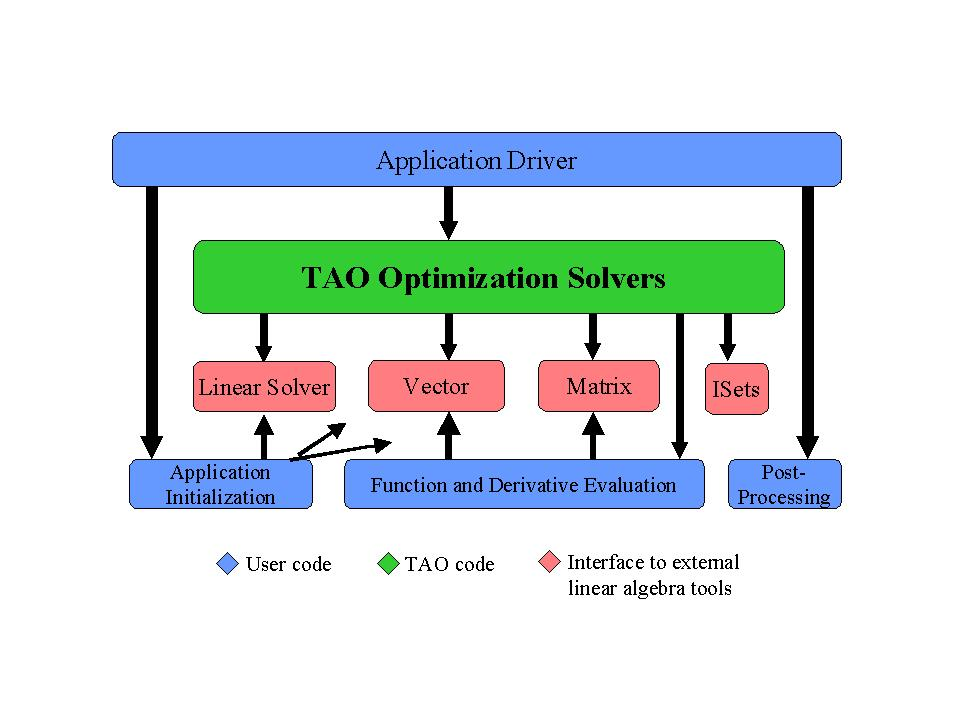
\includegraphics[height=2.5in]{../images/tao_pic3}}
\else
\fi

\vfill

\end{slide}

\begin{slide}
\heading{Using PETSc Objects on Multiple Processors}

\begin{alltt}
\scriptsize \setlength{\baselineskip}{8pt}
  TAO_SOLVER      tao;              /* TAO Optimization solver          */
  TAO_APPLICATION app;              /* TAO Application using PETSc      */
  AppCtx          user;             /* user-defined application context */
  \textcolor{red}{Vec             x;               /* solution vector                  */
  Mat             H;                /* Hessian Matrix                   */

  VecCreateMPI(PETSC_COMM_WORLD,n,&x);}
  \textcolor{red}{MatCreateAIJ(PETSC_COMM_WORLD,nlocal,nlocal,n,n,d_nz,d_nnz,o_nz,o_nnz,&H);}
  TaoCreate(\textcolor{red}{PETSC_COMM_WORLD},TAOLMVM,&tao);
  TaoApplicationCreate(\textcolor{red}{PETSC_COMM_WORLD},&app);
  TaoAppSetInitialSolutionVec(app,x);
  TaoAppSetObjectiveRoutine(app,\textcolor{blue}{FormFunction,(void *)&user});
  TaoAppSetGradientRoutine(app,\textcolor{blue}{FormGradient,(void *)&user});
  TaoAppSetHessianMat(app,H,H);
  TaoAppSetHessianRoutine(app,\textcolor{blue}{FormHessian,(void *)&user});
  TaoSolveApplication(app,tao);
  VecView(x,\textcolor{red}{PETSC_VIEWER_STDOUT_WORLD});
\end{alltt}

\vfill

\end{slide}


\begin{slide}

\heading{Convergence}

\vfill

\end{slide}


\begin{slide}

\heading{TAO Basic Facilities}

\begin{list}{\reddiamond}{}
\item
TaoAppSetInitialSolutionVec
\item
TaoAppSetVariableBounds
\item
TaoGetLinearSolver
\item 
TaoFromOptions
\item
TaoAppSetMonitor
\item
TaoView
\item
\ldots
\end{list}

\vfill

\end{slide}

% \begin{slide}
% \heading{Where Can We Find TAO?}
% 
% At {\bf http://www.mcs.anl.gov/tao}
% 
% \begin{list}{\reddiamond}{\leftmargin=1in}
% \item
% Source Code
% \item
% Documentation
% \item
% Installation Instructions
% \item
% Example Problems
% \item
% Additional Tutorials
% \item
% Performance Results
% \item
% Supported Architectures
% \end{list}
% 
% \vfill
% 
% \end{slide}


\end{document}


\begin{slide}

\heading{}

\begin{list}{\reddiamond}{}
\item

\end{list}

\vfill

\end{slide}

\begin{slide}

\heading{Optimization Toolkits}

State-of-the-art in optimization software:

\begin{list}{\reddiamond}{}
\item
Scattered support for parallel computations
\item
Little reuse of linear algebra software
\item
Minimal use of automatic differentiation software
\item
Rigid assumptions about data representations
\item
Nonlinear optimization problems with more than $ 10, 000 $
variables are considered large.
\end{list}

\vfill

\end{slide}

\begin{slide}

\heading{TAO}

The process of nature by which all things change
and which is to be followed for a life of harmony.

\bigskip

\begin{center}
\textcolor{red}{The Right Way}
\end{center}

\bigskip

Toolkit for Advanced Optimization

\begin{list}{\reddiamond}{}
\item
Object-oriented techniques
\item
Component-based interactions
\item
Leverage of existing parallel computing infrastructure
\item
Reuse of external toolkits
\end{list}

\vfill

\end{slide}

\begin{slide}

\heading{TAO Goals}

\begin{list}{\reddiamond}{}
\item
High performance
\item
Scalable parallelism
\item
Portability
\item
An interface independent of architecture
\end{list}

\vfill

\end{slide}

\begin{slide}

\heading{TAO Algorithms (partial list)}

\begin{list}{\reddiamond}
{ \setlength{\itemsep}{0pt}}
\item
Unconstrained optimization 
\begin{list}{\reddash}{}
\item
Conjugate gradient algorithms PR, FR, PR+
\item
Newton line search and trust region
\end{list}
\item
Bound-constrained optimization
\begin{list}{\reddash}{}
\item
Limited-memory variable-metric algorithm
\item
Trust region Newton method
% \item
% Gradient projection/conjugate gradient algorithm
\end{list}

\item Complementarity
\begin{list}{\reddash}{}
\item Semismooth methods
\end{list}
%\item
%Linearly constrained optimization
%\begin{list}{\reddash}{}
%\item
%Interior-point quadratic programming  method (alpha)
%\end{list}
\end{list}

\vfill

\end{slide}
